
\documentclass[a1paper,portrait]{baposter}

\usepackage[utf8]{inputenc}
\usepackage{amsmath, amssymb}
\usepackage{graphicx}
\usepackage{multicol}
\usepackage{color}

\definecolor{darkgreen}{RGB}{0,100,0}
\definecolor{darkblue}{RGB}{0,0,120}

\begin{document}

\begin{poster}{
  columns=3,
  colspacing=1em,
  background=plain,
  eyecatcher=true,
  headerborder=closed,
  borderColor=darkgreen,
  headerColorOne=darkgreen,
  headerColorTwo=darkblue,
  headerFontColor=white,
  boxColorOne=white,
  boxColorTwo=white,
  headershape=roundedright,
  headerfont=\Large\bf\textsf,
  textborder=roundedleft,
  linewidth=2pt
}
% Eye catcher (top left)
{}
% Title
{\bf\textsf{Lemniscata de Penin ($\infty\!\!\diagup$) --- Evolução Infinita sob Trilhos}}
% Authors
{\textsf{Daniel Penin, 2025}}
% Logo (top right)
{}

% Motivaçao
\headerbox{Motivação}{name=motivation,column=0,row=0}{
\begin{itemize}
\item ET$\Omega$: poderosa, mas complexa, dependente de $\gamma$ e $\lambda$.
\item Necessidade de evolução contínua + segura sem parâmetros frágeis.
\item Surge o conceito: \textbf{Infinito sob Trilhos}.
\end{itemize}
}

% Definição
\headerbox{Definição da Equação}{name=definition,column=1,row=0}{
\begin{center}
\Large
$P = \infty\!\!\diagup(E + N - iN)$ \\[1ex]
\normalsize
$iN = (1 - I)N, \quad I \in [0,1]$
\end{center}
\begin{itemize}
\item $E$: Eficiência útil
\item $N$: Novidade informativa
\item $iN$: Novidade inadmissível
\item $I$: Integridade
\end{itemize}
}

% Simulação
\headerbox{Simulação}{name=simulation,column=2,row=0}{
\begin{itemize}
\item Comparação de 300 iterações:
\begin{enumerate}
\item Sistema $\infty\!\!\diagup$: progresso estável.
\item Baseline sem trilhos: instabilidades e colapsos.
\end{enumerate}
\end{itemize}
\begin{center}
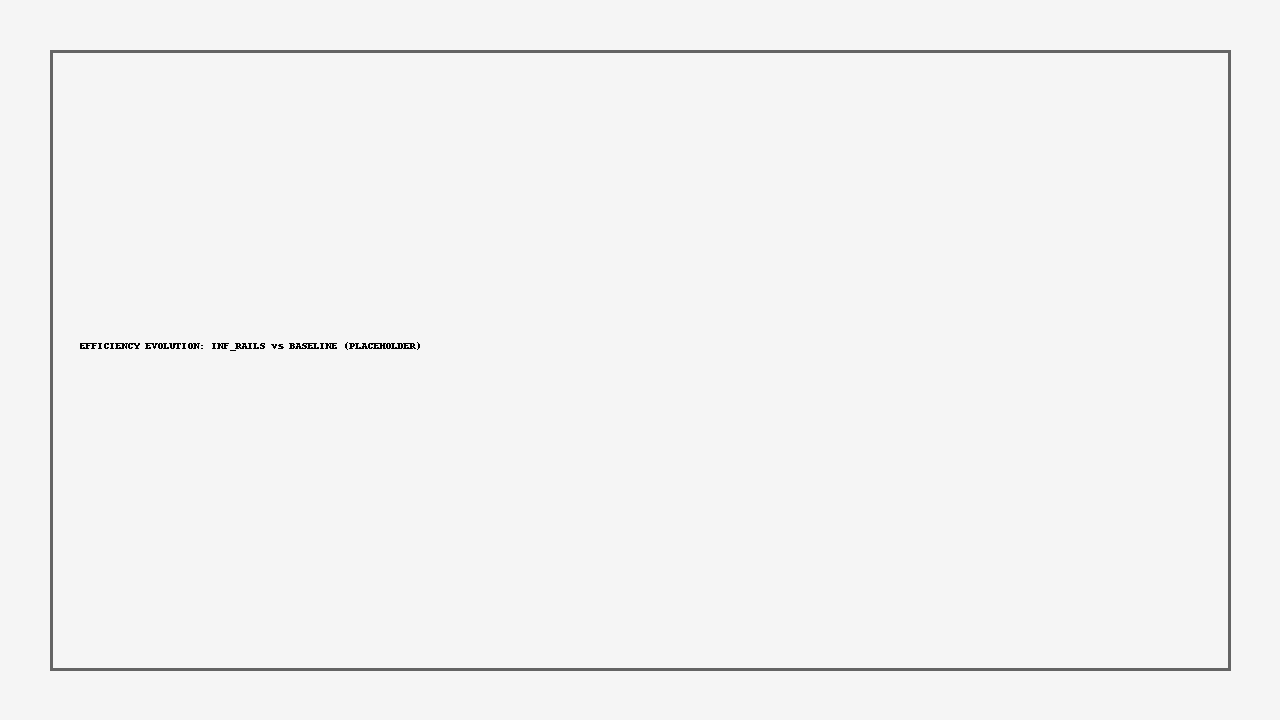
\includegraphics[width=0.8\linewidth]{figures/efficiency_placeholder.png}
\end{center}
}

% Aplicações
\headerbox{Aplicações}{name=applications,column=0,below=motivation}{
\begin{itemize}
\item IA evolutiva segura
\item Multiagente colaborativo
\item Integração quântica
\item Robótica, saúde, cibersegurança
\end{itemize}
}

% Impacto
\headerbox{Impacto Histórico}{name=impact,column=1,below=definition}{
\begin{itemize}
\item Simplicidade comparável a $E=mc^2$
\item Símbolo próprio ($\infty\!\!\diagup$)
\item Paradigma para a era da inteligência artificial
\end{itemize}
}

% Conclusão
\headerbox{Conclusão}{name=conclusion,column=2,below=simulation}{
\begin{itemize}
\item \textbf{Infinito, mas sob trilhos.}
\item Evolução infinita + integridade.
\item Potencial de valor histórico e científico.
\end{itemize}
}

\end{poster}
\end{document}
